\chapter{试样加工及研究方法设计}
\section{材料属性与试样加工过程}
\subsection{实验材料属性}
本实验用的是真空自耗两次熔炼所得的钛合金板,其化学成分参数与室温(20℃)力学性能参数如\ref{sec:mytc4chem}与\ref{sec:mytc4machin}所示:
\begin{table}[htbp]
	\centering
	\caption{试样的化学成分参数}
	\label{sec:mytc4chem}
	\begin{tabular}{cccccccc}
		\toprule
		元素($ \% $) & Al & V &Fe &C& O& N &H \\ \midrule
		实际含量 & 6.12&4.06 &0.13 &0.012&0.112&0.009&0.004  \\
		标准要求 &$ 5.5\sim 6.75 $ & $ 3.5\sim 4.5 $&$ \le 0.30 $ & $ \le 0.05 $&$ \le 0.20 $&$ \le 0.03$ &$ \le 0.015 $ \\ \bottomrule
	\end{tabular}
\end{table}
\begin{table}[htbp]
	\centering
	\caption{试样的力学性能参数}
	\label{sec:mytc4machin}
	\begin{tabular}{cccc}
		\toprule
		力学性能& 抗拉强度$Mpa  $& 屈服强度$ Mpa $&断后伸长率$ \% $\\ \midrule
		实测值 & 983 &902 & 13\\
		标准值 &$ \ge 895 $&$ \ge 830 $&$ \ge 10 $ \\ \bottomrule
	\end{tabular}
\end{table}

%
%\begin{figure}[!htbp]
%	\centering
%	\begin{minipage}[t]{0.68\textwidth}
	%		\centering
	%		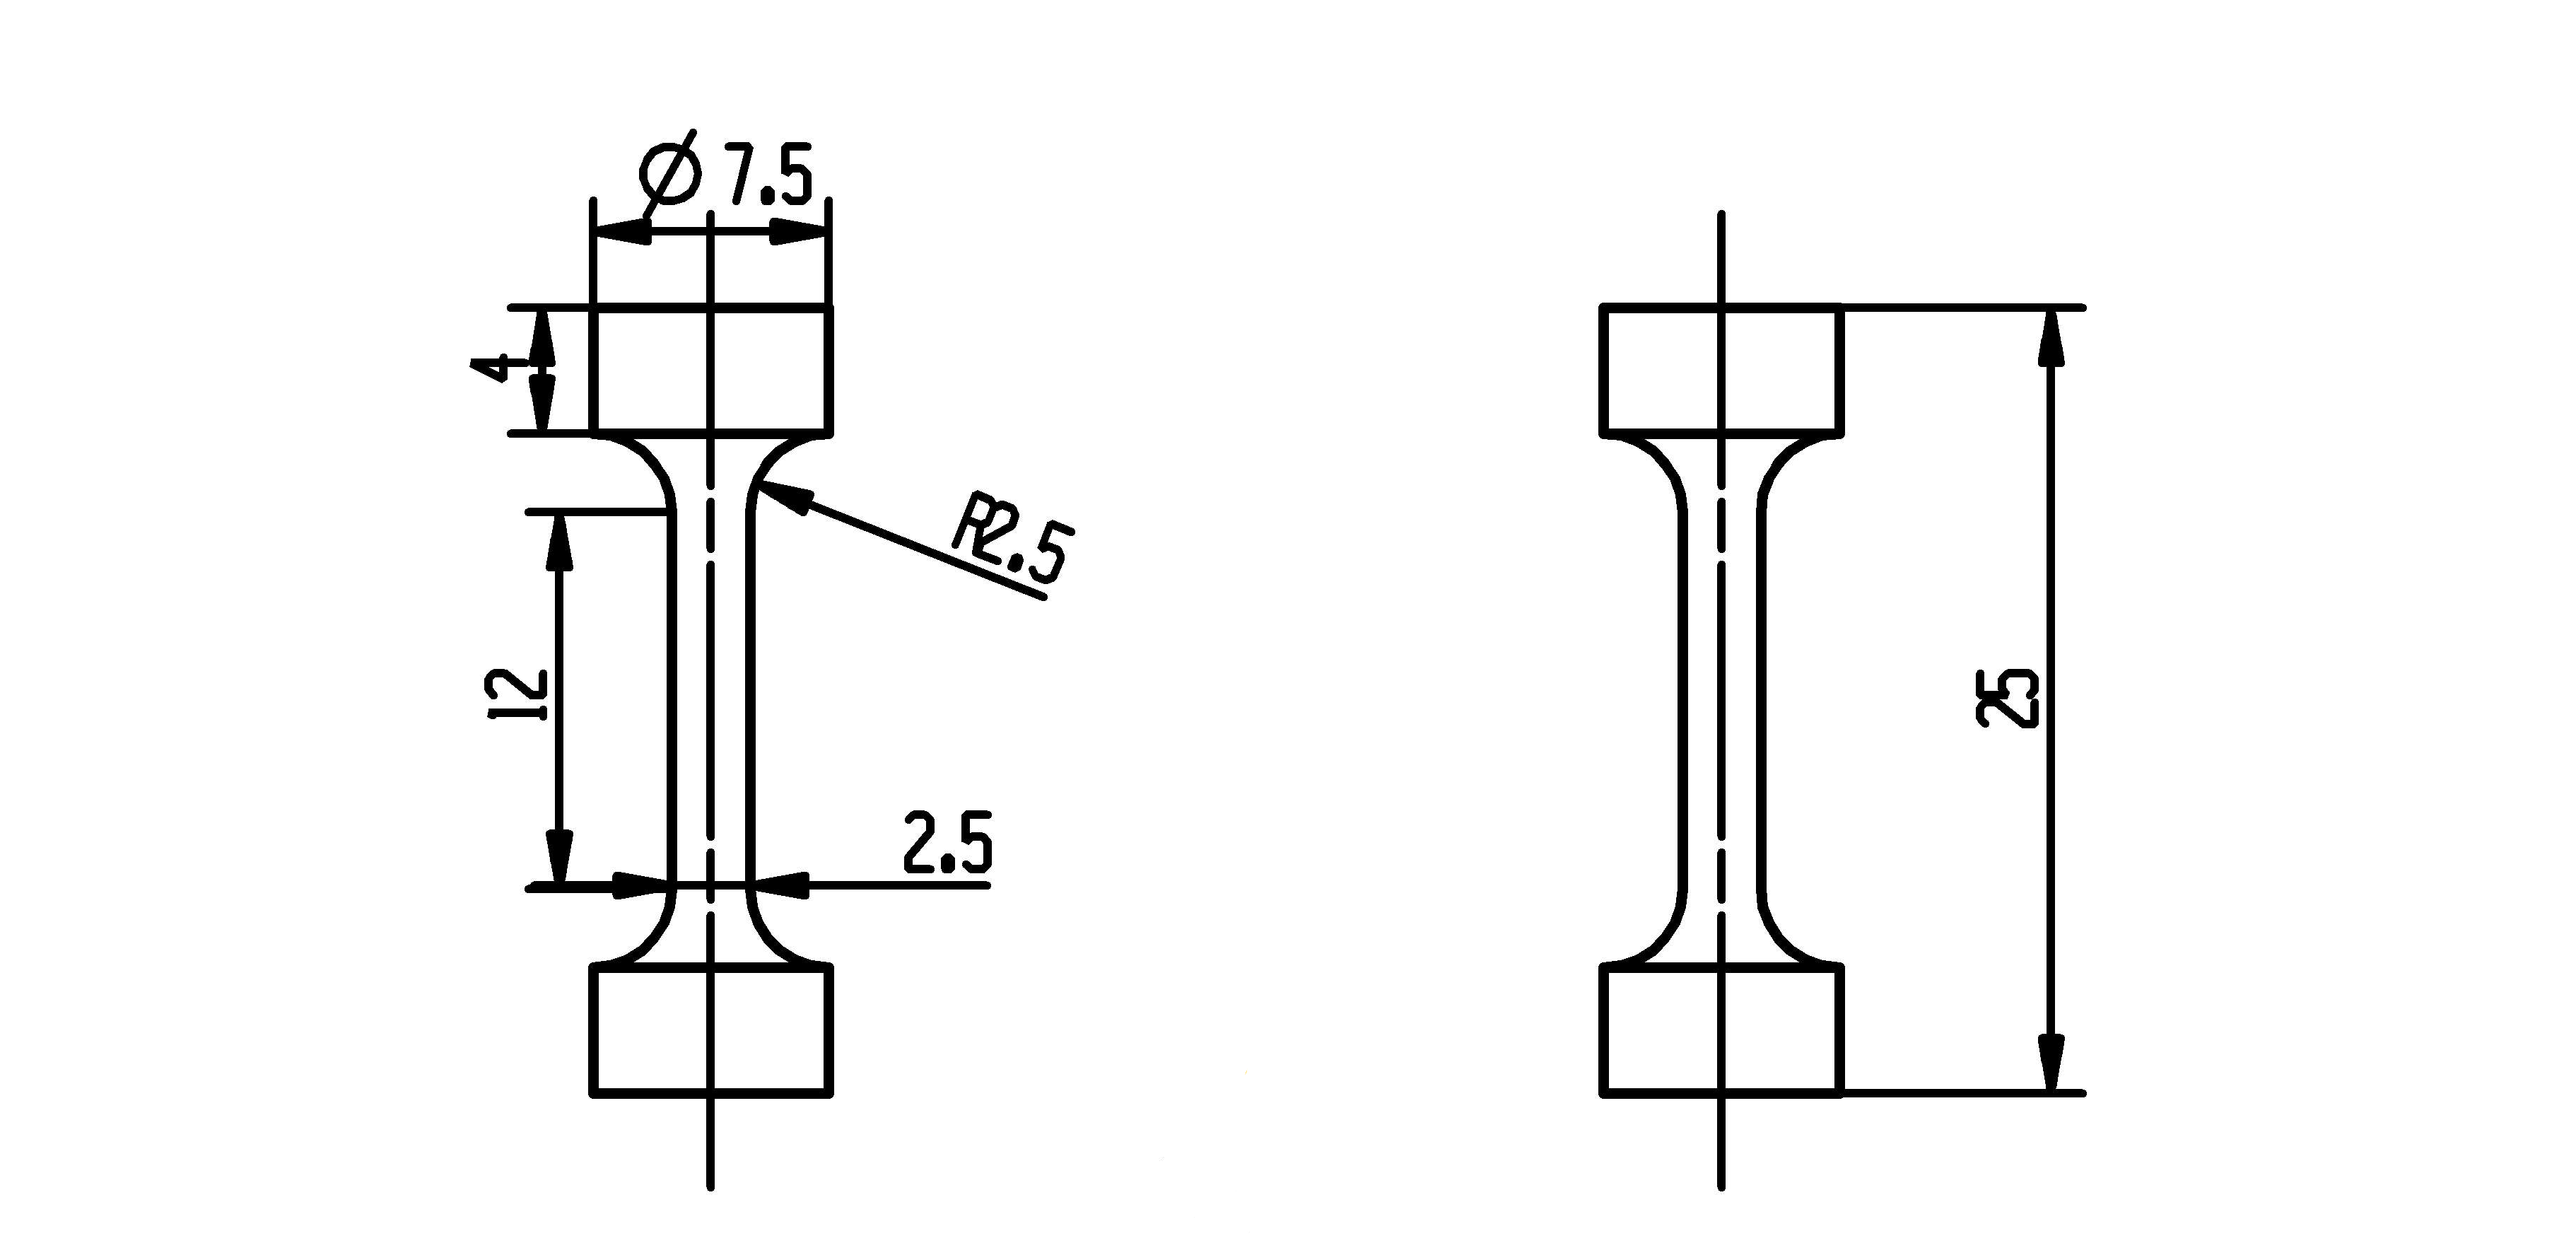
\includegraphics[width=6cm]{pic/试样}
	%		\caption{试样的尺寸参数}
	%		\label{fig:试样尺寸}
	%	\end{minipage}
%	\begin{minipage}[t]{0.3\textwidth}
	%		\centering
	%		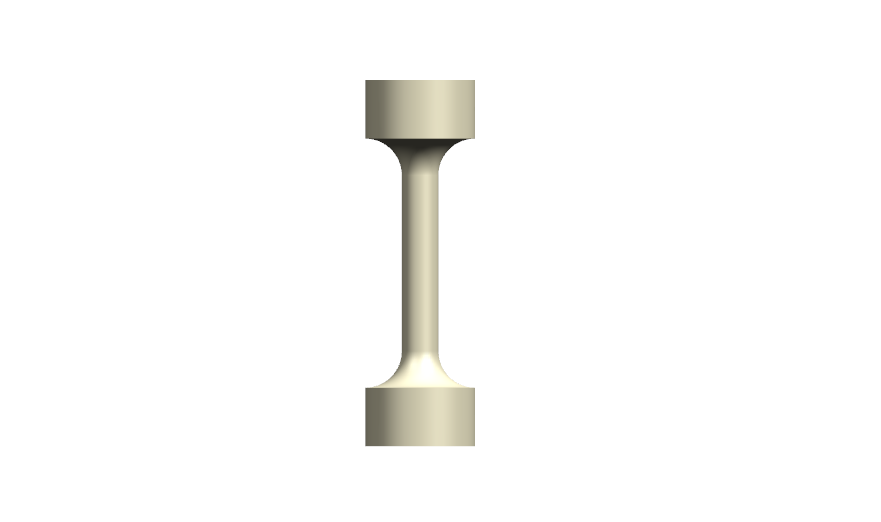
\includegraphics[width=6cm]{pic/模型}
	%		\caption{试样的三维模型}
	%		\label{fig:试样的三维模型}
	%	\end{minipage}
%%	\caption{试样参数}
%\end{figure}

\subsection{$\beta$转变温度的计算}
$\beta$转变温度是钛合金的重要参数之一,它是制定钛合金的热机械工艺和热处理工艺的重要依据,相变过程如\ref{sec:Tc4betachange}所示。

\begin{table}[htbp]
	\centering
	\caption{\ti 合金$ \alpha+\beta \to \beta $转变时发生的相变及存在的相}
	\label{sec:Tc4betachange}
	\begin{tabular}{ccc}
		\toprule 室温相 & 相变过程 & 高温相 \\
		\midrule$\alpha-\mathrm{Ti}$ & $\alpha-T i \rightarrow \beta-T i$ & $\beta-\mathrm{Ti}$ \\
		$\alpha-\mathrm{Ti}-\mathrm{Al}$ & $\alpha-\mathrm{Ti}-\mathrm{Al} \rightarrow \beta-\mathrm{Ti}+\beta-\mathrm{Ti}-\mathrm{Al}$ & $\beta-\mathrm{Ti}, \beta-\mathrm{Ti}-\mathrm{Al}$ \\
		$\beta- \mathrm{Ti}-\mathrm{V}$ & $\beta-\mathrm{Ti}-\mathrm{V} \rightarrow \beta^{-} \mathrm{Ti}-\mathrm{V}$ & $\beta-\mathrm{Ti}-\mathrm{V}$ \\
		\bottomrule
	\end{tabular}
\end{table}

$\beta$转变温度于TC4合金组织转变的关系非常密切,对于TC4合金热处理工艺的设计至关重要。郭凯\cite{guokaiTC4taihejinrechuligongyideyanjiuxianzhuangjijinzhan2021}等人表示:当固溶温度高于 $\beta$ 相变时的温度时,合金的强度伴随温度的增加而下降,而且残余应力也开始大幅度的降低;当固溶温度在相变点以下时,合金的强度伴随温度的增加而增加。但是徐戊矫、谭玉全\cite{xujianGurongshixiaogongyiduiTC4taihejinzuzhijixingnengdeyingxiang2014}却表明:在相变点以下,随着退火温度的升高,材料的 强度、塑性和冲击韧性呈降低趋势。之所以会出现这种完全相反的结论,很可能是研究者对于相变点的具体值定义不清晰导致的,可见相变点的确定在固溶处理过程中是非常关键的。


关于$\beta$转变温度的具体值,目前广泛认同的是位于975℃附近,但是由于不同试样的合金元素的种类与含量的差异,尤其是局部化学成分的差异,使得不同研究人员实际测得的相变点温度有所差异\cite{wangtaoTC4hejinxiangbianwendujiancezhongjieguobuyizhiyuanyinfenxi2013}。姚德人等\cite{yaoderenTc4taihejinxiangbiandiandeceding1975}表明相变温度为975℃到980℃之间,此时的合金拥有最低的硬度,当温度略大时会发生$\beta$晶粒的显著长大;相变点以下50℃以内水淬,可以得到不同数量的初生$ \alpha $和马氏体$ \alpha^{\prime} $,而后再进行低温退火时,马氏体$ \alpha^{\prime} $又会转变为稳定的次生$ \alpha$和$ \beta $,可以得到较好的综合性能\footnote{\color{black}此文章写于1975年,但是仍然非常有参考价值}。刘伟东等人\cite{liuweidongTC4hejinVzhuanbianwendudejinxiangfacedingyulilunjisuan2014}通过连续升温金相法,使用EET\footnote{Empirical Electron Theory of solids and molecules“固体与分子经验电子理论”(简称余氏理论)}模型建模测得了\ti 合金的相变温度为974.58℃;孙宇、曾卫东等人\cite{sunyuYingyongrengongshenjingwangluoyanjiuhuaxueyuansuduitaihejinxiangbiandiandeyingxiang2010}通过人工神经网络ANN技术,运用反向传播算法,建立了三层神经网路-钛合金相变预测模型,最终预测得到在绝对误差为9.8℃的情况下,TC4的相变点为994.8℃。

近年来,确定$ \beta $相变点的常见计算方法\cite{zhuhongTaihejinaVxiangbiandiandejizhongceshifangfatantao2013}主要有:连续升温金相法、X 射线衍射法、电阻法、等热膨胀法、元素含量法和神经网络模型预测预测法\cite{renchiqiangGurongshixiaoduiTC4taihejinxianweizuzhihelixuexingnengdeyingxiang2022}等。其中元素含量法是最为常用的方法,简单且准确。该方法根据合金中各元素对相变温度的影响\cite{ananyaLocationBasedIntelligent2011}利用经验公式\ref{jingyan}来对相变点进行推算:
\begin{equation}
	T_\beta=885^{\circ} \mathrm{C}+\sum \textit{ 各元素含量 } \times \textit{ 各元素含量对 }(\alpha+\beta) / \beta \textit{ 相变点的影响 }
	\label{jingyan}
\end{equation}
其中885℃为纯钛的相变点。

故本设计采用元素含量法来对实验材料的$\beta$转变温度进行推算,元素含量如上\ref{sec:mytc4chem}所示,不同元素对于相变点温度的影响如\ref{sec:chem4ti}所示:
\begin{table}[htbp]
	\centering
	\caption{部分元素含量对钛合金相变点的影响}
	\label{sec:chem4ti}
	\begin{tabular}{cccc}
		\hline 元素名称 & 元素含量 $(\mathrm{Wt} \%)$ & 差值&累积值 \\
		\hline $\mathrm{Al}$ & $2.0 \sim 7.0$ & 29+$23.0^{\circ} \mathrm{C} / 1.0 \%$ & $+123.76^{\circ} \mathrm{C}$ \\
		$\mathrm{V}$ & $0 \sim 10.0$ & $-14.0^{\circ} \mathrm{C} / 1.0 \%$ & $-56.84^{\circ} \mathrm{C}$ \\
		$\mathrm{Fe}$ & $0 \sim 15.0$ & $-16.5^{\circ} \mathrm{C} / 1.0 \%$ & $-2.145^{\circ} \mathrm{C}$
		 \\
		$\mathrm{C}$ & $0 \sim 0.15$ & $+2.0^{\circ} \mathrm{C} / 0.01 \%$ &$ +2.4^{\circ} \mathrm{C} $\\
		$\mathrm{O}$ & $0 \sim 1.0$ & $+2.0^{\circ} \mathrm{C} / 0.01 \%$& $ +22.4^{\circ} \mathrm{C} $\\
		$\mathrm{~N}$ & $0 \sim 0.5$ & $+5.5^{\circ} \mathrm{C} / 0.01 \%$& $ +4.95^{\circ} \mathrm{C} $\\
		$\mathrm{H}$ & $0 \sim 0.50$ & $-5.5^{\circ} \mathrm{C} / 0.01 \%$ &$ -2.2^{\circ} \mathrm{C} $\\
		\hline
	\end{tabular}
\end{table}

\begin{equation}
\begin{aligned}
T_\beta&=885^{\circ} \mathrm{C}+\sum (\delta_{Al}+\delta_{V}+\delta_{Fe}+\delta_{C}+\delta_{O}+\delta_{N}+\delta_{H})\\
&= 885^{\circ} \mathrm{C}+(123.76-56.84-2.145+2.4+22.4+4.95-2.2)^{\circ} \mathrm{C}\\
&=885^{\circ} \mathrm{C}+92.325^{\circ} \mathrm{C}\\
&=977.325^{\circ} \mathrm{C}
\end{aligned}
\end{equation}

最终通过计算法得到的相变点温度为$977.325^{\circ} \mathrm{C} $,与广泛认同的相变点温度值相差$\delta=\frac{977.325-975}{975}=0.238\% $,可见还是比较符合现实情况的,故本实验选择此温度作为热处理实验的基准温度。


\subsection{试样设计与加工}
本设计选择了尺寸较小的试样来进行实验:整体尺寸为$ 25mm\times 7.5mm $,厚度为1.3mm,呈现为两端略大,中间平行的骨头状。该类型的小件试样不仅可以节约材料,特殊的形状也便于进行后续的力学拉伸试验,满足实验要求,十分适合于昂贵金属的试验。参数如\ref{fig:试样尺寸}所示:
%3-28日上午,经过老师说明,由于试样为板材,加工成圆柱较为困难,故加工成二位平面的“狗骨头”

\begin{figure}[h!]
	\centering
	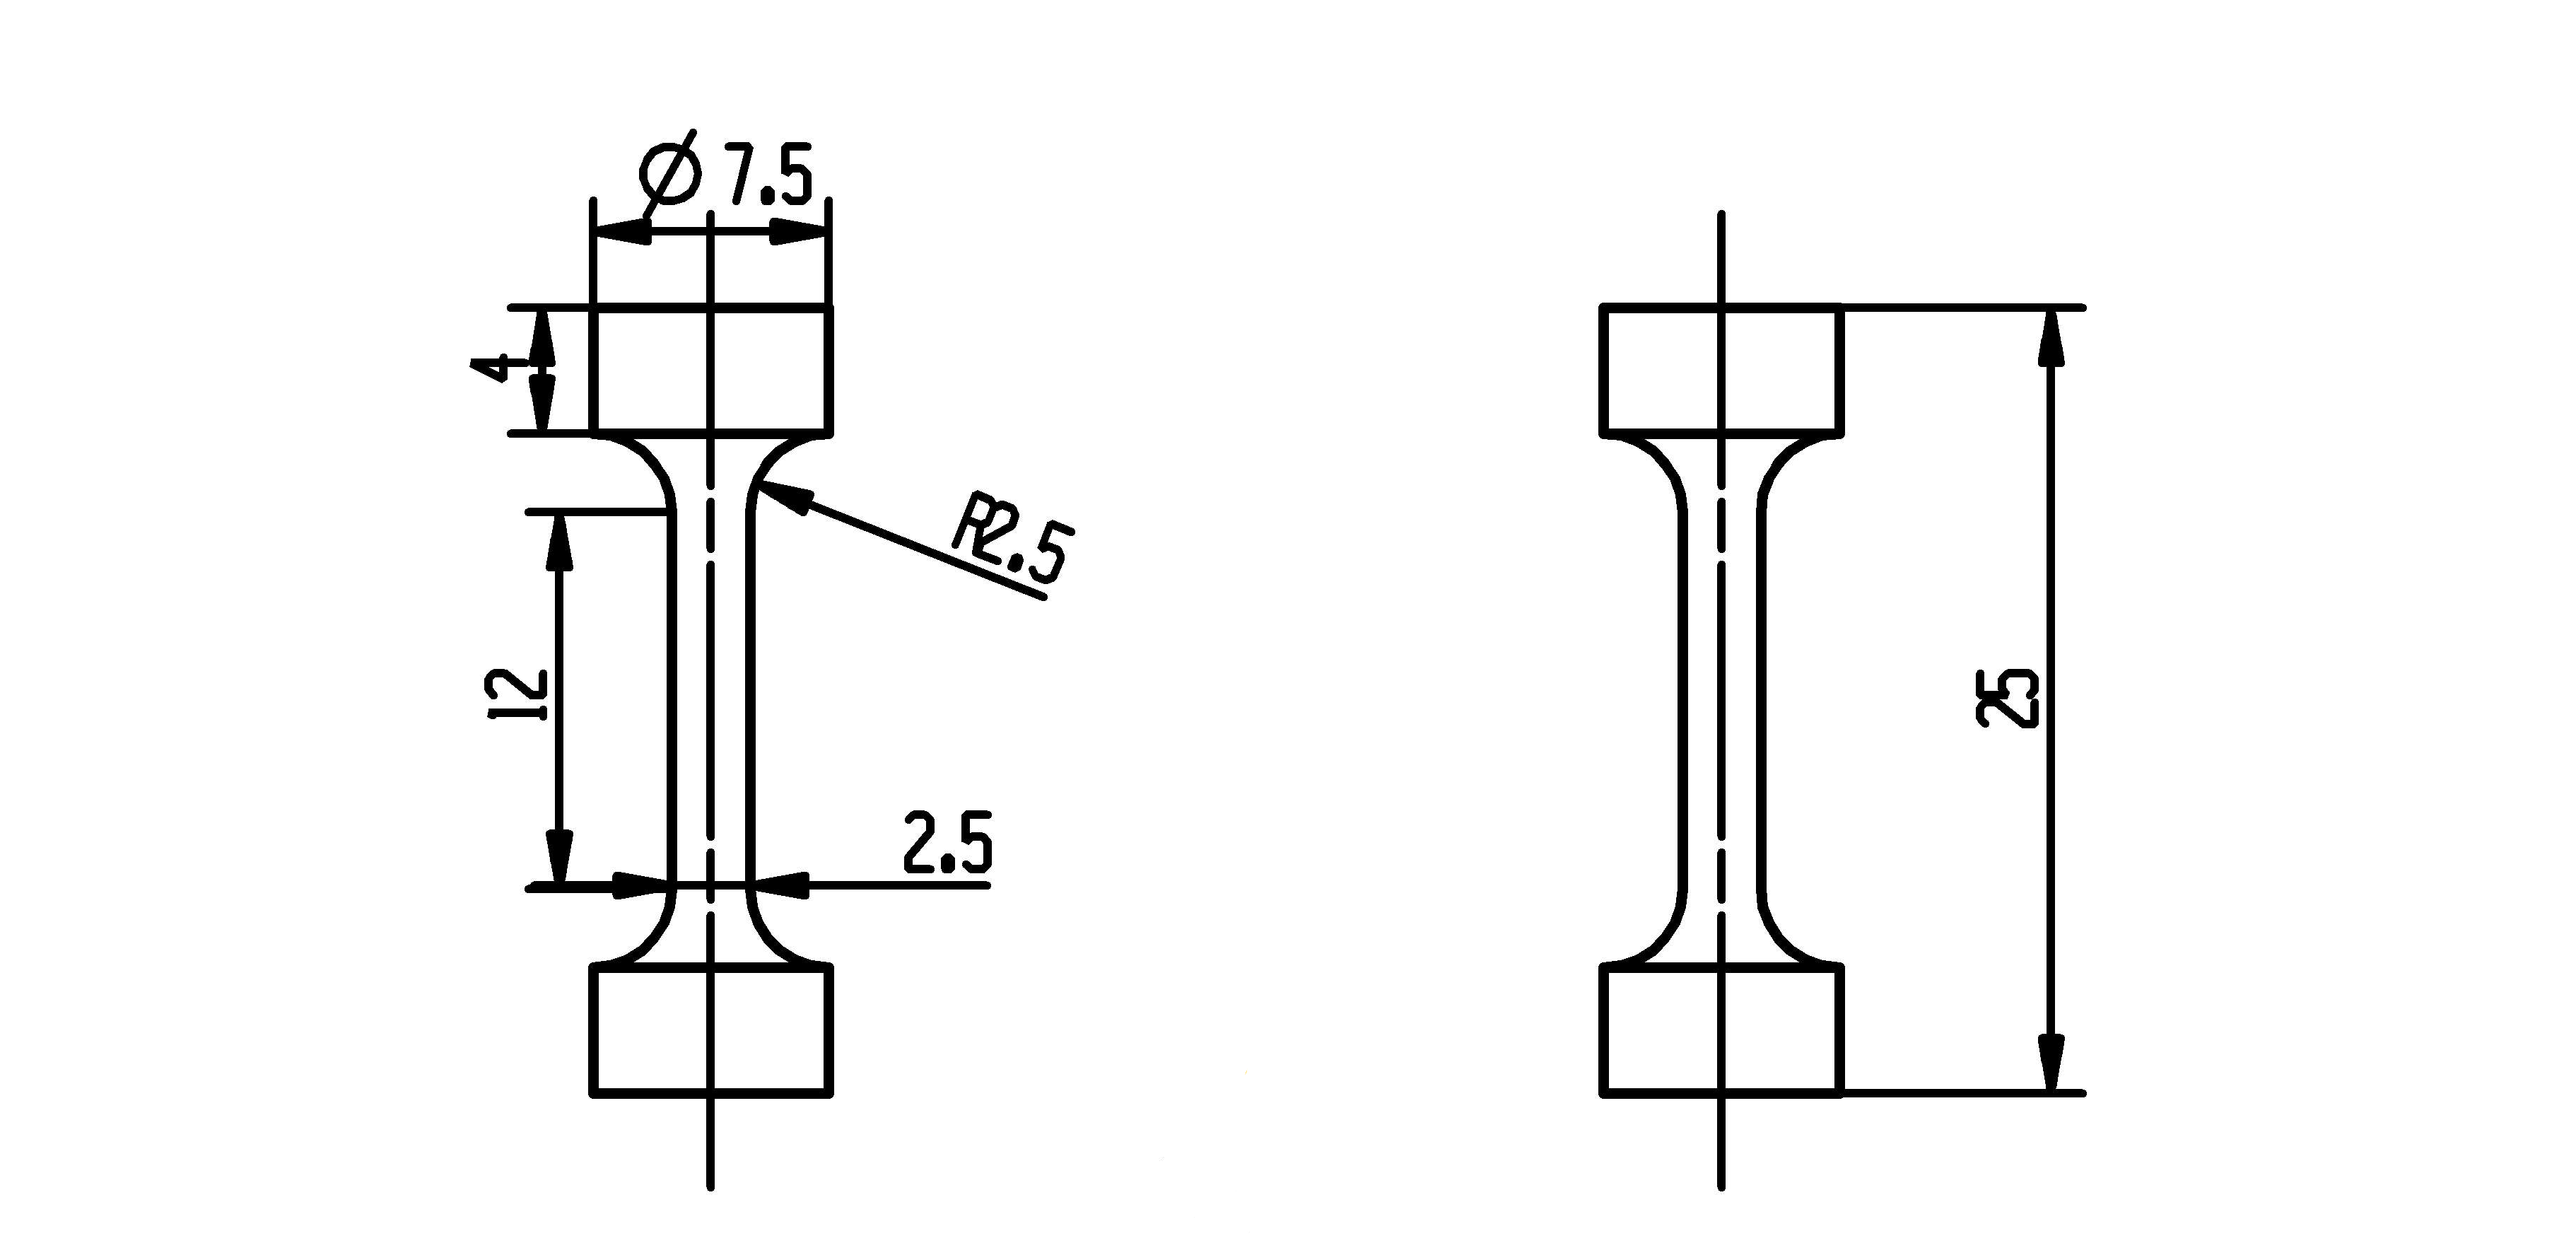
\includegraphics[width=0.7\linewidth]{pic/试样}
	\caption{试样的尺寸参数}
	\label{fig:试样尺寸}
\end{figure}

原始的材料板材$ 250\time 150 $(mm)的板材,为了加工出来目标形状的试样,本设计选用电火花线切割(Wire cut Electrical Discharge Machining)的方法进行加工。

在一开始只考虑了材料的利用率,就设计了如\ref{fig:badway}所示的密集排列。但是在实际加工的时候,却发现在这样的设计方式根本不可行——没有夹具的位置,且刀路比较长。
\begin{figure}[h!]
	\centering
	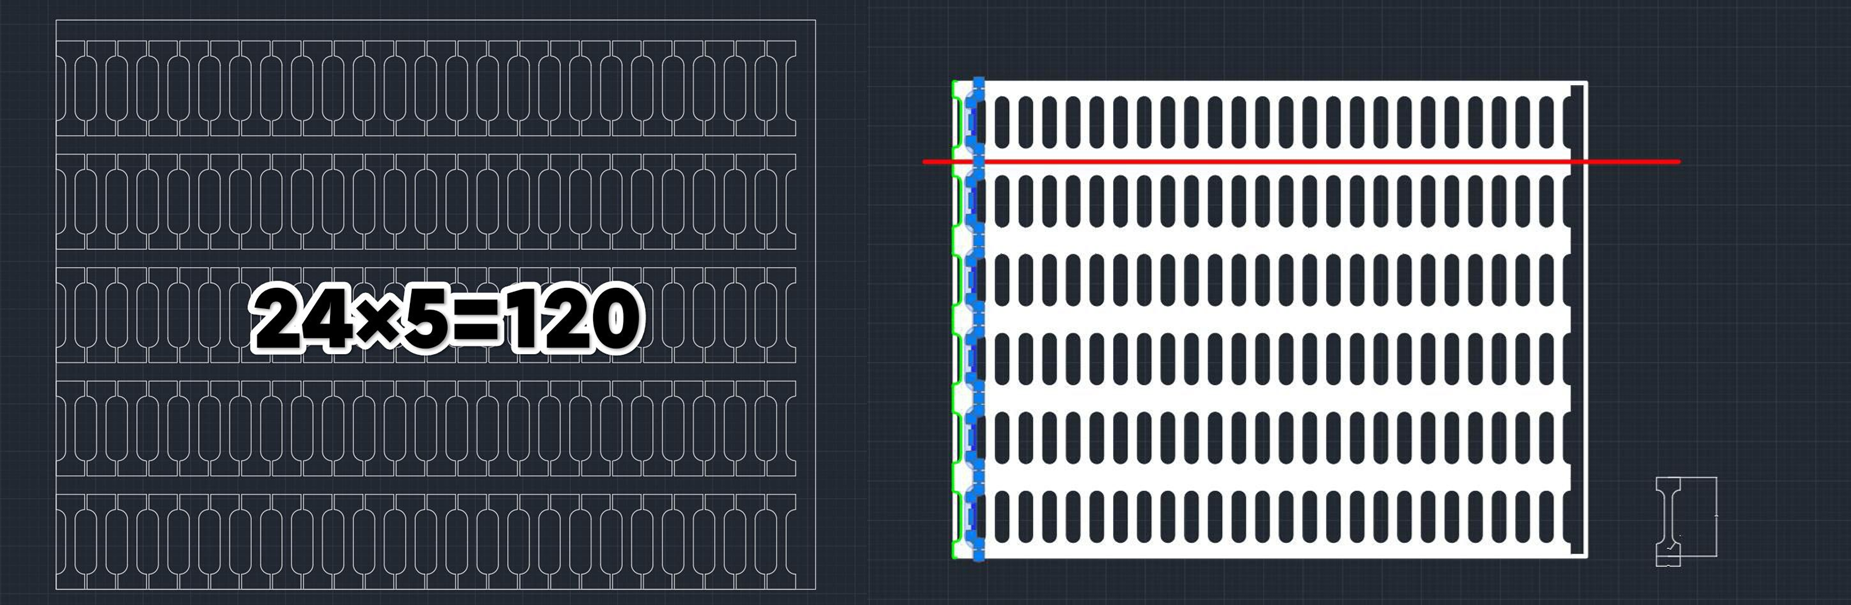
\includegraphics[width=0.8\linewidth]{pic/刀路初步}
	\caption{初步设计的刀路}
	\label{fig:badway}
\end{figure}

在仔细考虑了加工方法、设备特点、加工成本等因素后,在工程训练中心张冠老师的协助下,将加工方式改进成了:先把大板切割成八个小板,再把小板叠在一起进行加工的方法,最终切割出来了$ 7\times 8=56 $个试样。
\begin{figure}[h!]
	\centering
	\subfigure[堆叠式切割]{
		\label{fig:goodway}
		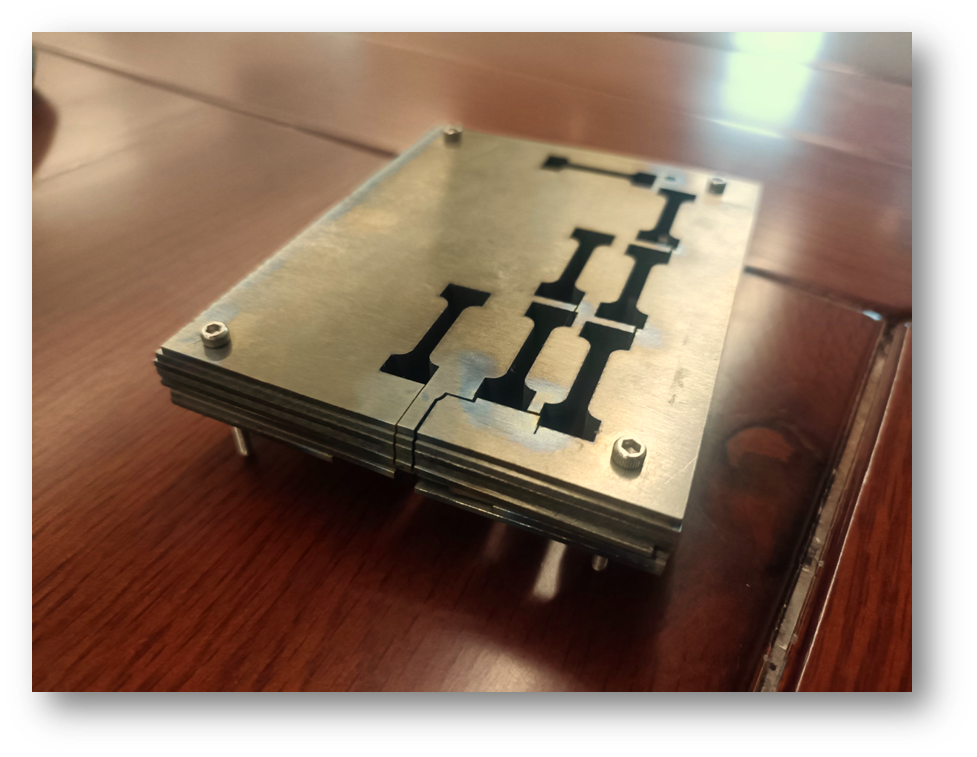
\includegraphics[width=0.4\linewidth]{pic/堆叠式切割}}
	\hspace{0.2in} % 两图片之间的距离
	\subfigure[切割结果]{
	\centering
		\label{fig:mytc4bone}
		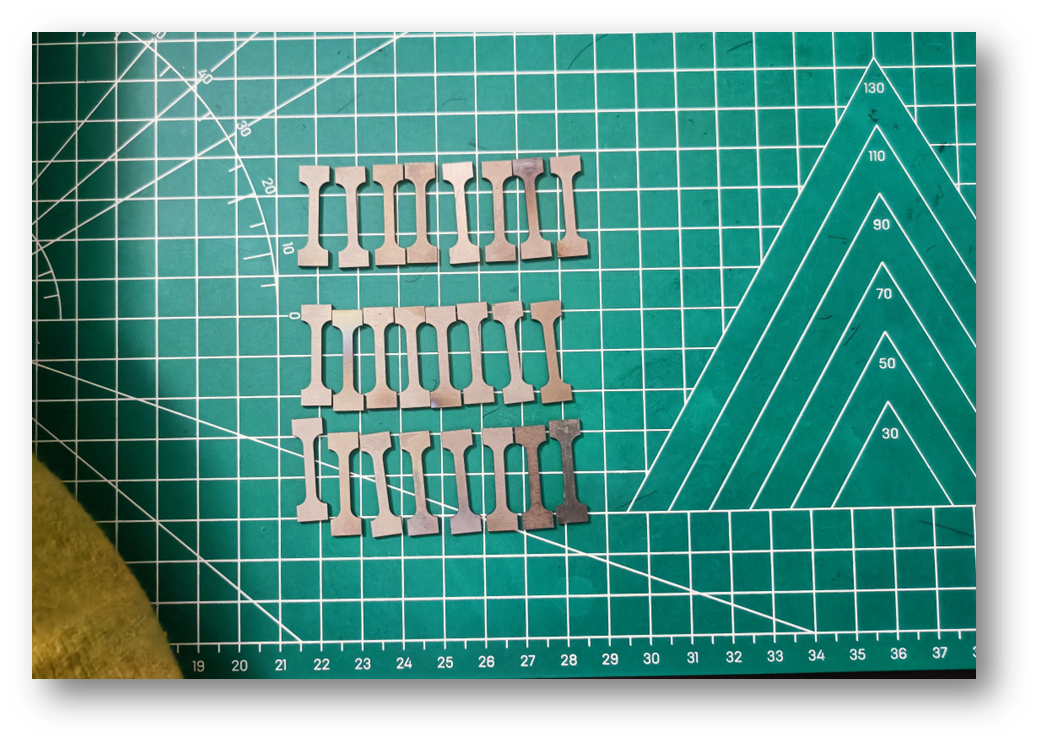
\includegraphics[width=0.45\linewidth]{pic/切割后的试样}}
		\caption{切割方法与切割结果}
\end{figure}

\section{TC4钛合金的热处理方案设计}
\subsection{TC4合金的热处理工艺性能}
由~\ref{sec:1.1}可知,钛合金可以通过各种各样的相变过程来得到不同的组织结构。因而可以设计适宜的热处理工艺参数,来获得具有高强度的显微组织,由此实现\ti 合金力学性能和工艺性能的改善。\ti 合金热处理的一些特性如下:
\begin{enumerate}
	%	\item 钛合金的热处理主要用于$\alpha+\beta$型钛合金。因为对于纯α型钛合金而言,马氏体相变不会使钛合金的性能发生显著变化。只能依赖淬火形成的亚稳相(包括马氏体相)的时效分解来进行。
	%	\item 热处理应该避免形成ω相。形成ω相会使钛合金变脆,正确选择时效工艺(例如,采用较高的时效温度)即可使相分解。
	\item $\alpha+\beta$钛合金的淬透性差,淬火热应力大,淬火时零件易翘曲。由于导热性差,钛合金变形时易引起局部温升过高,使局部温度有可能超过$\beta$转变点而形成魏氏组织。
	\item 化学性质活泼。热处理时,钛合金易与氧和水蒸气反应,在工件表面形成具有一定深度的富氧层或氧化皮,使合金的性能降低。同时钛合金热处理时容易吸氢,引起氢脆。
	\item $\beta$转变点差异大。即使是同一成分,但由于冶炼炉次的不同,其$\beta$转变温度有时差别很大。
\end{enumerate}
\subsection{TC4合金热处理工艺设计}
常见的\ti 钛合金热处理工艺有:退火、淬火(往往加上时效处理)、形变热处理等,不同的热处理方式得到的组织性能各异。

鲁媛媛,马保飞等人研究发现在时效温度为450℃、500℃和550℃时初生α相的含量随温度升高逐渐增加;而在时效温度为600℃和650℃条件下初生$\alpha$相含量因高温溶解而明显减少, $\beta$相尺寸相应增大。当时效温度为550℃时, 所得钛合金的显微组织最佳\cite{luyuanyuanShixiaochuliduiTC4taihejinweiguanzuzhihelixuexingnengdeyingxiang2019}。刘婉颖、林元华等人通过实验发现:在960 ℃/1 h + WQ进行固溶处理和500 ℃/4 h + AC下进行时效处理得到的\ti 具有最佳的力学性能\cite{LiuWanYingBuTongReChuLiGongYiDuiTi6Al4VTaiHeJinWeiGuanJieGouHeLiXueXingNengYingXiangYingWen2017};陈冠宇通过实验表明,在850℃进行退火处理时,在600℃进行时效处理可以使合金得到更好的耐腐蚀性能\cite{1200};李宸宇证明\ti 合金在900℃空冷固溶两小时在530℃时效四小时后具有更好的强硬度,而且固溶后冷速越快,合金的强硬度越高、塑韧性越差\cite{900}。%第46页

总之,对于$\alpha+\beta$型的\ti 钛合金的固溶时效热处理工艺而言,其主要影响参数为温度和时间\cite{mirror1,ranxingGurongwenduduiTi6Al4VELItaihejinxianweizuzhijixingnengdeyingxiang2021}。根据初步预测确定了固溶处理的最佳工艺制度为$ \beta $相变点以下30℃左右(这里取整数$ 977.325-30=947.325\approx950^{\circ} \mathrm{C} $)处理一个小时、时效温度在450℃左右处理一个小时。于是本设计设置了如下三个变量:固溶温度、固溶方式、时效温度。根据控制变量法,设计了如\ref{sec:first}所示的18组热处理实验:
\begin{table}[htbp]
	\centering
	\caption{\ti 原本的热处理制度设计}
	\label{sec:first}
	\begin{tabular}{cccccc}
		\toprule
		固溶温度/℃ &处理时间/h & 冷却方法 & 时效温度/℃  &处理时间/h & 冷却方法 \\
		\midrule
		910 & 1 & $\mathrm{WQ}$ & 510 & 4 & $\mathrm{AC}$\\
		910 & 1 & $\mathrm{FC}$  & 510 & 4 & $\mathrm{AC}$ \\
		910 & 1 & $\mathrm{WQ}$ & 550 & 4 & $\mathrm{AC}$ \\
		910 & 1 & $\mathrm{FC}$  & 550 & 4 & $\mathrm{AC}$ \\
		910 & 1 & $\mathrm{WQ}$ & 590 & 4 & $\mathrm{AC}$ \\
		910 & 1 & $\mathrm{FC}$  & 590 & 4 & $\mathrm{AC}$ \\
		\midrule
		950 & 1 & $\mathrm{WQ}$ & 510 & 4 & $\mathrm{AC}$ \\
		950 & 1 & $\mathrm{FC}$ & 510 & 4 & $\mathrm{AC}$ \\
		950 & 1 & $\mathrm{WQ}$ & 550 & 4 & $\mathrm{AC}$ \\
		950 & 1 & $\mathrm{FC}$ & 550 & 4 & $\mathrm{AC}$ \\
		950 & 1 & $\mathrm{WQ}$ & 590 & 4 & $\mathrm{AC}$ \\
		950 & 1 & $\mathrm{FC}$ & 590 & 4 & $\mathrm{AC}$ \\
		\midrule
		990 & 1 & $\mathrm{WQ}$ & 510 & 4 & $\mathrm{AC}$ \\
		990 & 1 & $\mathrm{FC}$ & 510 & 4 & $\mathrm{AC}$ \\
		990 & 1 & $\mathrm{WQ}$ & 550 & 4 & $\mathrm{AC}$ \\
		990 & 1 & $\mathrm{FC}$ & 550 & 4 & $\mathrm{AC}$ \\
		990 & 1 & $\mathrm{WQ}$ & 590 & 4 & $\mathrm{AC}$ \\
		990 & 1 & $\mathrm{FC}$ & 590 & 4 & $\mathrm{AC}$ \\
		\bottomrule
	\end{tabular}
\end{table}


\subsection{优化实验设计}
控制变量法是科学实验中最常使用的方法,在面对低因素、低水平的实验时可以设计出很清晰直观的实验。但其也存在巨大的缺点,尤其是多个因素交互作用的影响,面对多因素(变量)、多水平的实验时,就需要设计很多次的实验,显得极为繁琐。比如一个含有三个变量,每个变量有三个水平的实验就需要$ 3\times 3 \times 3=27$次实验,为了直观性而牺牲大量的成本、同时包含了太多无关的对照组,这样的实验设计在很大程度上是不符合可持续发展理念的,是在浪费资源。但好在有另外一种方法可以解决问题——正交试验设计法(Orthogonal experimental design)。

正交实验设计是研究多因素多水平的又一种设计方法,可以用更少的试验次数来研究多个变量之间的关系。它是根据正交性从全面试验中挑选出部分有代表性的点进行试验,这些有代表性的点具备了“均匀分散,齐整可比”的特点\cite{wangxueshen}。当实验次数太多时,根据正交实验设计,实验者可以选择一部分有代表性水平组合进行试验。 例如前面说的三因素三水平的实验,若按$ L9(3^4) $正交表安排实验,只需作9次,按$ L15(3^7) $正交表进行15次实验,就可以大大减少试验次数,提高实验效率、材料利用率。


在没有通过正交实验设计优化之前,笔者的实验是如\ref{sec:first}所示,需要做$3\times2\times3  =18$次实验。但为了给子孙后代留下天蓝、地绿、水清的美丽家园,本实验高举可持续发展理念伟大旗帜,结合了正交实验方法$\color{black} L9.3.4 $对实验进行了优化。\\
最终的热处理制度如下表所示:%\footnote{其中WQ表示水冷、FC表示炉冷、AC表示空冷。}
\begin{table}[htbp]
	\centering
	\caption{\ti 改进后的热处理制度}
	\label{sec:myHT}
	\resizebox{\linewidth}{!}{
\begin{tabular}{ccccccc}
	\toprule
		实验编号&固溶温度/℃ &处理时间/h & 冷却方法 & 时效温度/℃  &处理时间/h & 冷却方法 \\
	\midrule
	1 & 910 & 1 & 水冷 & 510 & 1 & AC \\
	2 & 910 & 1 & 油冷 & 590 & 1 & AC \\
	3 & 910 & 1 & 水冷 & 550 & 1 & AC \\
	4 & 950 & 1 & 水冷 & 590 & 1& AC \\
	5 & 950 & 1 & 水冷 & 550 & 1& AC \\
	6 & 950 & 1 & 油冷 & 510 & 1 & AC \\
	7 & 990 & 1 & 水冷 & 550 & 1 & AC \\
	8 & 990 & 1 & 油冷 & 510 & 1 & AC \\
	9 & 990 & 1 & 水冷 & 590 & 1 & AC \\
%	910 & 1 & $\mathrm{WQ}$ & 510 & 4 & $\mathrm{AC}$\\
%	910 & 1 & $\mathrm{FC}$  & 510 & 4 & $\mathrm{AC}$ \\
%	910 & 1 & $\mathrm{WQ}$ & 550 & 4 & $\mathrm{AC}$ \\
%	910 & 1 & $\mathrm{FC}$  & 550 & 4 & $\mathrm{AC}$ \\
%	910 & 1 & $\mathrm{WQ}$ & 590 & 4 & $\mathrm{AC}$ \\
%	910 & 1 & $\mathrm{FC}$  & 590 & 4 & $\mathrm{AC}$ \\
%	\midrule
%	950 & 1 & $\mathrm{WQ}$ & 510 & 4 & $\mathrm{AC}$ \\
%	950 & 1 & $\mathrm{FC}$ & 510 & 4 & $\mathrm{AC}$ \\
%	950 & 1 & $\mathrm{WQ}$ & 550 & 4 & $\mathrm{AC}$ \\
%	950 & 1 & $\mathrm{FC}$ & 550 & 4 & $\mathrm{AC}$ \\
%	950 & 1 & $\mathrm{WQ}$ & 590 & 4 & $\mathrm{AC}$ \\
%	950 & 1 & $\mathrm{FC}$ & 590 & 4 & $\mathrm{AC}$ \\
%	\midrule
%	990 & 1 & $\mathrm{WQ}$ & 510 & 4 & $\mathrm{AC}$ \\
%	990 & 1 & $\mathrm{FC}$ & 510 & 4 & $\mathrm{AC}$ \\
%	990 & 1 & $\mathrm{WQ}$ & 550 & 4 & $\mathrm{AC}$ \\
%	990 & 1 & $\mathrm{FC}$ & 550 & 4 & $\mathrm{AC}$ \\
%	990 & 1 & $\mathrm{WQ}$ & 590 & 4 & $\mathrm{AC}$ \\
%	990 & 1 & $\mathrm{FC}$ & 590 & 4 & $\mathrm{AC}$ \\
	\bottomrule
\end{tabular}
}
\end{table}

%\subsection{正交实验分析方法}
%经过正交实验方法设计的实验虽然节省了试验次数,但是不能兼顾直观性,因而需要专门的分析工具才能分析出来,不同变量之间的相关性,故本实验采用spssau提供的数据分析工具来对三因素影响结果进行分析。

%{\Huge \color{red} \textbf {待补充}}

\section{TC4钛合金的热处理方案实验过程}
按照\ref{sec:myHT}设置好的工艺,本实验分先后两次进行热处理:先进行固溶处理,随后进行时效处理,方案路线如\ref{fig: heatway}所示。
\begin{figure}[h!]
	\centering
	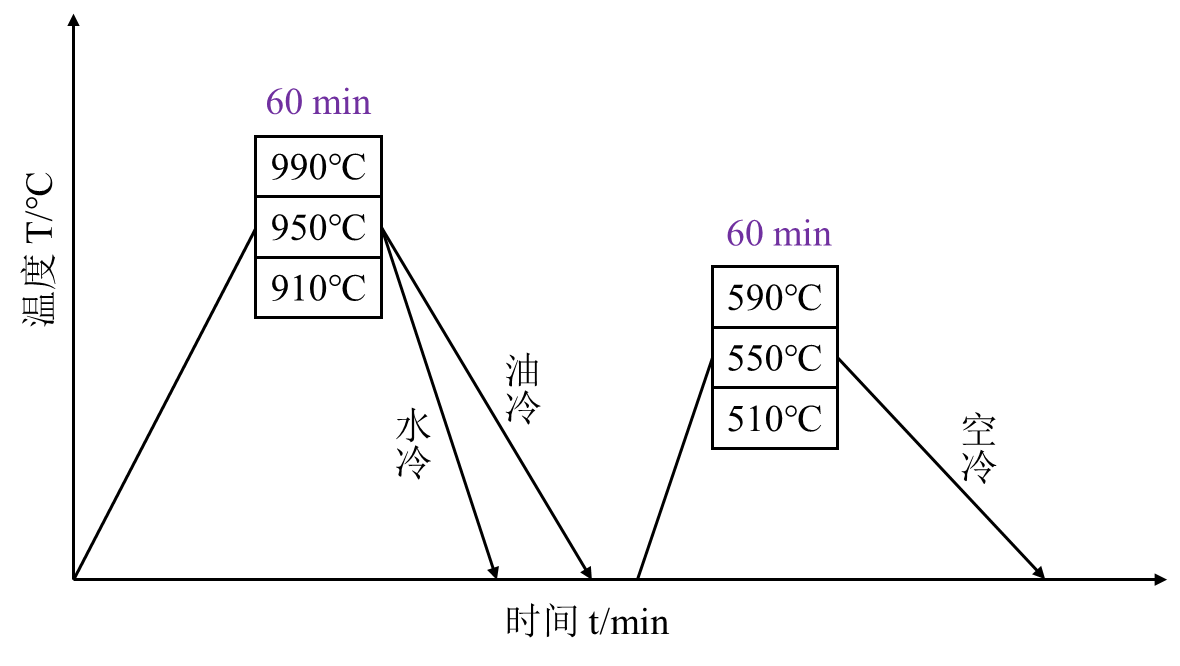
\includegraphics[width=0.7\linewidth]{pic/处理路线}
	\caption{固溶-时效热处理试验路线}
	\label{fig: heatway}
\end{figure}
\subsection{实验设备}
本次设计热处理实验所用的设备为\text{\color{teal}JC-MF12-30}型箱式电阻炉,外观如\ref{fig: mymuffle}所示,设备规格如\ref{sec:mymuffle}所示:


\begin{table}[htbp]
	\centering
	\caption{\text{\color{teal}JC-MF12-30}型箱式电阻炉的规格}
	\label{sec:mymuffle}
		\begin{tabular}{cc}
			\toprule
			参数&值\\
			\midrule
			型号&JC-MF12-30\\
			编号&803229\\
			电压&380V\\
			功率&12KW\\
			常用温度&1150℃\\
			最高温度&1200℃\\
			炉膛尺寸& 500$ \times $ 300$ \times $ 200(mm) \\
			制造日期&2023年2月\\
			制造商& $\text{青岛聚创}^\text{\textregistered}  $环保集团有限公司\\
			\bottomrule
		\end{tabular}
\end{table}

\begin{figure}[h!]
	\centering
	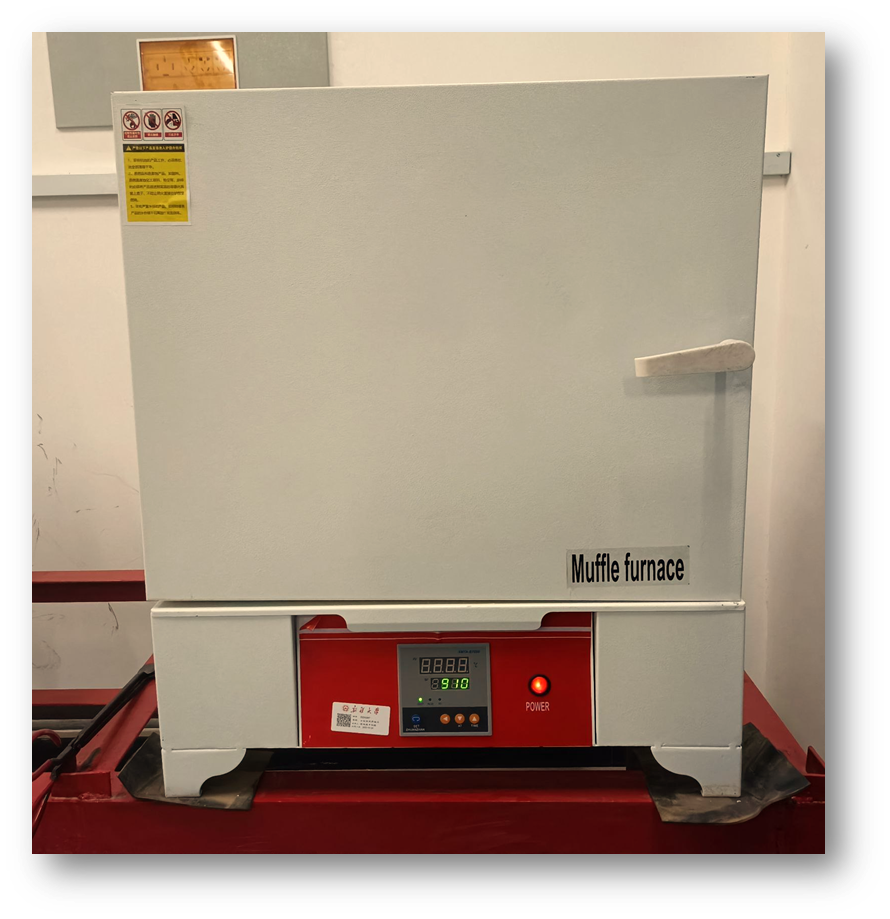
\includegraphics[width=0.6\linewidth]{pic/马弗炉}
	\caption{马弗炉外形}
	\label{fig: mymuffle}
\end{figure}

固溶实验需要淬火,用到的淬火液体如\ref{fig:淬火用液体}所示:
\begin{figure}[h!]
	\centering
	\subfigure[水淬液]{
		\label{fig:subfig:WCfluid}
		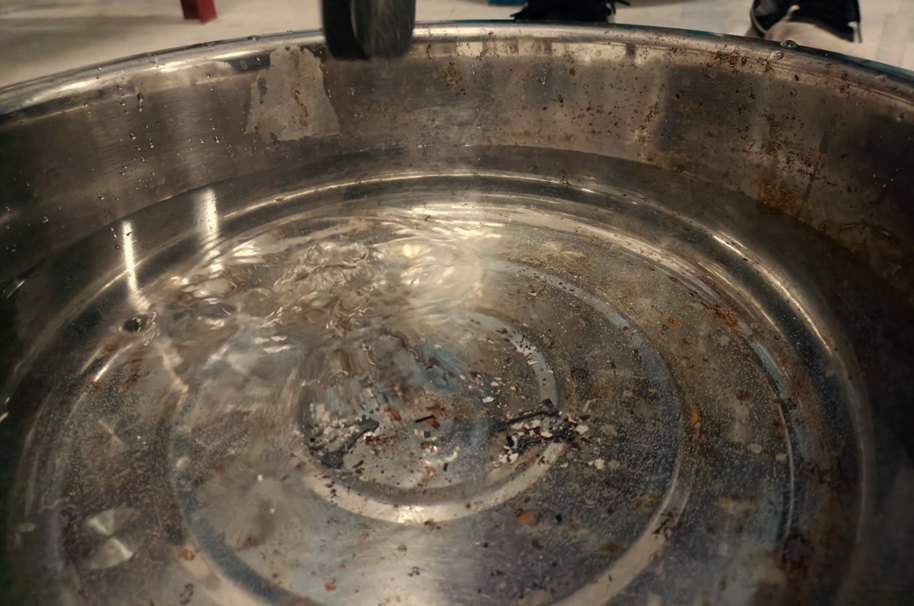
\includegraphics[scale=0.4]{pic/水淬液}}
	\hspace{0.5in} % 两图片之间的距离
	\subfigure[淬火油]{
		\label{fig:subfig:OCfluid}
		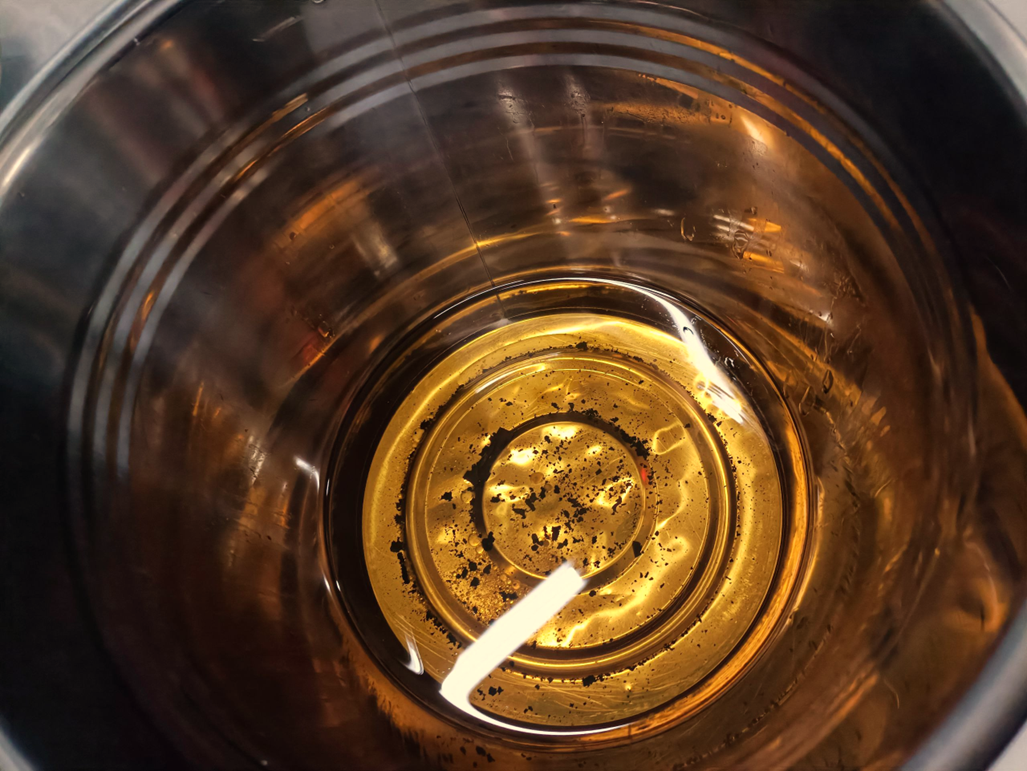
\includegraphics[scale=0.32]{pic/淬火油}}
	\caption{淬火用的液体}
	\label{fig:淬火用液体}
\end{figure}

\subsection{固溶处理实验过程}
\begin{enumerate}
	\item 设备与试样准备:把样品用去离子水等清洗干净,确保表面干净无杂质,无水分。准备陶瓷样品架,以便样品可以均匀加热。准备好后,将热处理炉预热至900℃左右,并保持稳定。
	\item 样品装入:将切好的样品用放置在样品架上,不要使样品直接接触炉子底部或顶部,以免影响加热效果。并确保样品间距均匀,并记录好摆放顺序。
	\item 加热过程控制:将样品架或钛合金网放入炉中,启动加热程序。根据实验要求,控制加热速率、温度和保温时间等参数(这里分三批次\textbf{910-950-990},每批次六个试样进行处理)。
	\item 保温时间控制:加热到设计的温度后后,让试样保温一段时间,使其完全进入固溶状态。保持加热系统稳定,避免温度波动。
	\item 停止加热:当固溶处理时间{\footnote{由于试样过小,老师建议加热10分钟,这样既可以节约时间,也可达到其他实验者粗大试样一个小时的效果}}到达后,停止加热并关闭加热系统,取出处理好的试样。
	\item 水淬或油淬:将处理后的样品快速分别浸入水中、淬火油中进行淬火(每批次四个水淬,两个油淬)。
	\item 后处理:取出样品进行干燥、清洗、归类,并记录初步记录数据。
\end{enumerate}
经过固溶时效处理后的试样如图所示:

\begin{figure}[h!]
	\centering
	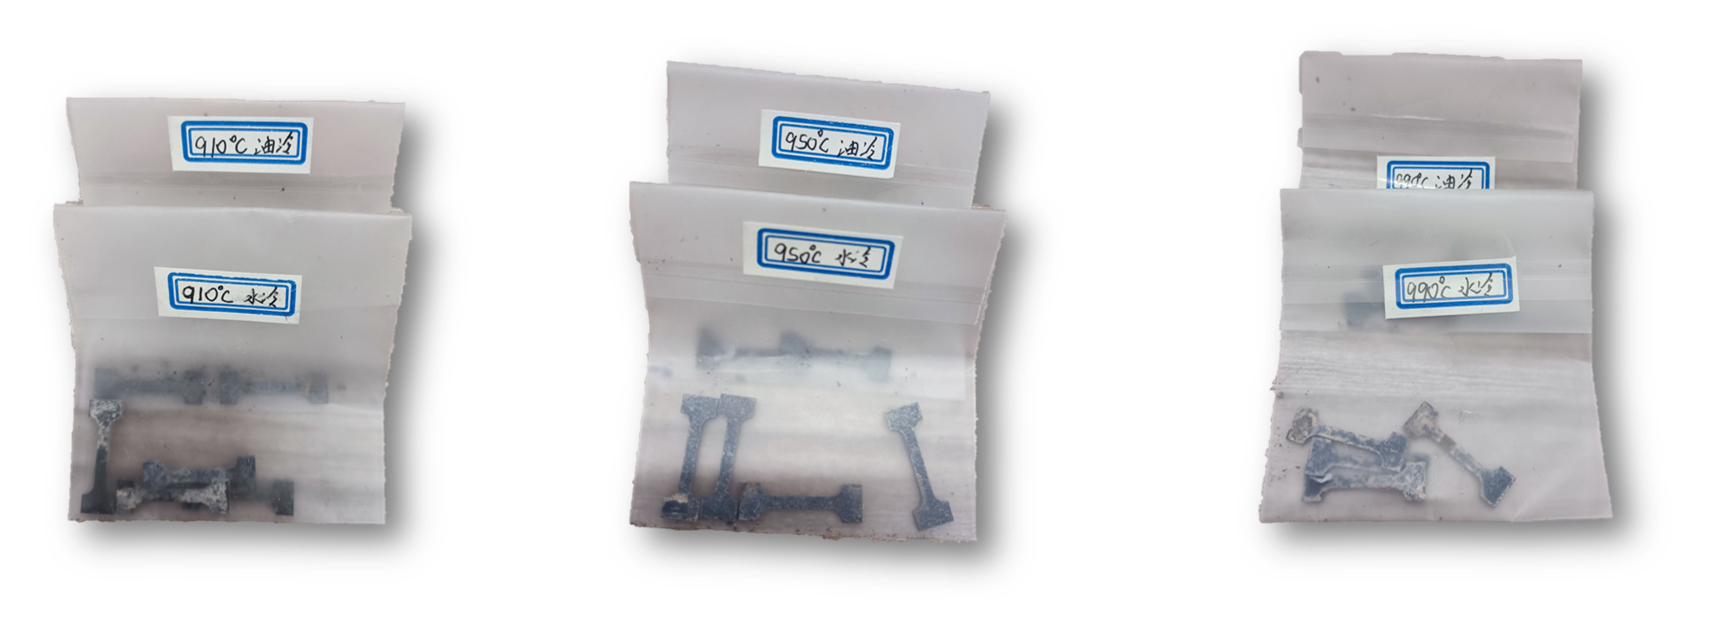
\includegraphics[width=0.8\linewidth]{pic/固溶处理后的试样}
	\caption{固溶处理后的试样}
	\label{fig: aftergurong}
\end{figure}

\subsection{时效处理实验过程}
时效处理过程温度稍低,为\textbf{510-550-590}三个温度,冷却方式为空冷,具体步骤与固溶处理相同,在此不做赘述。

处理后,使用砂纸将表面氧化层打磨干净,根据试样所处的不同工艺路线,将各个试样分组归类。

%\section{小结}
%在本节中,介绍了式样的参数与加工过程与热处理工艺的设计
